\documentclass[final,t]{beamer}
\mode<presentation>
{
  \usetheme{MCSposter}
  \usecolortheme{default}
  \usefonttheme[onlymath]{serif}
}
\usepackage[orientation=landscape,size=custom,width=120,height=90,scale=1.3]{beamerposter}
%\usepackage[orientation=landscape,size=a0,scale=1.4]{beamerposter}
\usepackage{pgfpages}
%\pgfpagesuselayout{resize to}[a4paper,landscape,border shrink=5mm]
%\pgfpagesuselayout{resize to}[a0paper,landscape]

% additional settings
\setbeamerfont{itemize}{size=\normalsize}
\setbeamerfont{itemize/enumerate body}{size=\normalsize}
\setbeamerfont{itemize/enumerate subbody}{size=\normalsize}

% additional packages
\usepackage{times}
\usepackage{subcaption}
\usepackage{textpos}
\usepackage{wrapfig}
\usepackage{sidecap}
%\usepackage{sfmath} 
\usepackage{amsmath,amsthm,bm,microtype}
\usepackage{siunitx}
\DeclareSIUnit\year{a}
\sisetup{retain-unity-mantissa = false}
\usepackage{exscale}
\usepackage{multicol,multirow}
\usepackage{booktabs}
%\usepackage[english]{babel}
\usepackage[latin1]{inputenc}
\newcommand\todo[1]{{\color{red}\bf [TODO: #1]}}
\usepackage{tikz}
\usetikzlibrary{decorations.pathreplacing}
\usetikzlibrary{shadows,arrows,shapes.misc,shapes.arrows,shapes.multipart,arrows,decorations.pathmorphing,backgrounds,positioning,fit,petri,calc,shadows,chains,matrix}
\usepackage{fancyvrb}
\newcommand\cverb[1][]{\SaveVerb[%
    aftersave={\textnormal{\UseVerb[#1]{vsave}}}]{vsave}}

\bibliographystyle{unsrt-shortauthor}

%\def\newblock{\hskip .11em plus .33em minus .07em} % for natbib and beamer IMPORTANT
\listfiles
\graphicspath{{/home/jed/talks/figures/}{/home/jed/src/aterrel-presentations/figures/}}
% Display a grid to help align images
%\beamertemplategridbackground[1cm]

\newcommand\jedcolor[1]{{}}

\title{\huge Parallel nonlinear solvers for viscoplastic models of sea ice {\normalsize \texttt{DI31A-2206}}}
\author[Jed Brown]{Jed Brown {\texttt{jedbrown@mcs.anl.gov}}}
\institute[MCS]{Download this poster from \url{http://59A2.org/files/201312-AGUSeaIce.pdf}}

\newcommand{\newt}[1]{\tilde{#1}}
\newcommand{\btab}{\hspace{\stretch{1}}}
\newcommand{\C}{\mathbb{C}}
\newcommand{\N}{\mathbb{N}}
\newcommand{\Q}{\mathbb{Q}}
\newcommand{\R}{\mathbb{R}}
\newcommand{\Rz}{\mathcal{R}}
\newcommand{\RR}{{\bar{\mathbb{R}}}}
\newcommand{\II}{\mathcal{I}}
\newcommand{\Z}{\mathbb{Z}}
\newcommand{\Zp}{\mathbb{Z}_+}
\newcommand{\B}{\mathcal{B}}
\newcommand{\M}{\mathcal{M}}
\newcommand{\LL}{\mathcal{L}}
\newcommand{\PP}{\mathscr{P}}
\newcommand{\ff}{\bm f}
\newcommand{\uu}{\bm u}
\newcommand{\vv}{\bm v}
\newcommand{\ww}{\bm w}
\newcommand{\DD}{D}
\newcommand{\EE}{\mathcal E}
\newcommand{\VV}{\bm{\mathcal{V}}}
\newcommand{\Pspace}{\mathcal{P}}
\newcommand\pfrak{{\mathfrak p}}
\newcommand{\di}{\partial}
\newcommand{\bigO}{\mathcal{O}}
\newcommand{\abs}[1]{\left\lvert #1 \right\rvert}
\newcommand{\bigabs}[1]{\big\lvert #1 \big\rvert}
\newcommand{\norm}[1]{\left\lVert #1 \right\rVert}
\newcommand{\ceil}[1]{\left\lceil #1 \right\rceil}
\newcommand{\floor}[1]{\left\lfloor #1 \right\rfloor}
\newcommand{\dif}{\bigtriangleup}
\newcommand{\ud}{\,\mathrm{d}}
\newcommand{\tcolon}{\!:\!}
\DeclareMathOperator{\sgn}{sgn}
\DeclareMathOperator{\card}{card}
\DeclareMathOperator{\trace}{tr}
\DeclareMathOperator{\sspan}{span}
\renewcommand{\bar}{\overline}
\newcommand{\ed}{\dot{\epsilon}}
\newcommand\citet[1]{\cite{#1}}
\newcommand\citep[1]{\cite{#1}}

% abbreviations
\usepackage{xspace}
\makeatletter
\DeclareRobustCommand\onedot{\futurelet\@let@token\@onedot}
\def\@onedot{\ifx\@let@token.\else.\null\fi\xspace}
\def\eg{{e.g}\onedot} \def\Eg{{E.g}\onedot}
\def\ie{{i.e}\onedot} \def\Ie{{I.e}\onedot}
\def\cf{{c.f}\onedot} \def\Cf{{C.f}\onedot}
\def\etc{{etc}\onedot}
\def\vs{{vs}\onedot}
\def\wrt{w.r.t\onedot}
\def\dof{d.o.f\onedot}
\def\etal{{et al}\onedot}
\makeatother
%%%%%%%%%%%%%%%%%%%%%%%%%%%%%%%%%%%%%%%%%%%%%%%%%%%%%%%%%%%%%%%%%%%%%%%%%%%%%%%%%%%%%%%%%%%%%%%%%%%%%%%%%%%%

% Need to declare these here because newcommand inside a frame is fragile
\newcommand\mgdx{1.9em}
\newcommand\mgdy{2.5em}
\newcommand\mgloc[4]{(#1 + #4*\mgdx*#3,#2 + \mgdy*#3)}
\newcommand{\mglevel}{\ensuremath{\ell}}
\newcommand{\mglevelcp}{\ensuremath{\mglevel_{\mathrm{cp}}}}
\newcommand{\mglevelfine}{\ensuremath{\mglevel_{\mathrm{fine}}}}

\begin{document}
\begin{frame}{} 
  \vspace{-3em}
  \begin{columns}
    \begin{column}{0.31\textwidth}
      \begin{block}{Sea ice dynamics}
         Sea ice variability plays an essential role in climate and is a hindrance to Arctic industries, yet current sea ice models have limited predictive capability and the underlying causes of the variability are not well understood.
         Despite being ``only'' a two-dimensional problem, the performance of the sea ice solver ranks alongside ocean and atmosphere as a leading bottleneck to scalability of earth system models.
         This difficulty is fundamental: the underlying physics of sea ice transmits information horizontally at the elastic wave speed of $v_p \approx \SI{3}{\kilo\metre\per\second}$, which is an order of magnitude faster than other components in a general circulation model.
         If this property of fast stress transmission is to be preserved in a sea ice model, the momentum solver must (provably) either perform many more neighbor communication steps or utilize multilevel solvers.
         % We present a parallel nonlinear (FAS) multigrid solver for visco-plastic rheology and compare it to existing methods in terms of robustness, scalability, and efficiency.
       \end{block}
       
      \begin{block}{Strong scaling challenges}
        Earth system modeling has a hard turn-around requirement of about 5 simulated years per day (SYPD) in order to perform the requisite science and still meet policy deadlines, including IPCC reporting.
        This requirement is equivalent to 47 seconds per simulated day, or $1825\times$ faster than real time.
        For high-resolution runs, CESM currently lags behind these objectives, due to limited parallelism and CFL constraints for transport processes.
        Sea ice currently runs \emph{sequentially} with atmosphere and the coupler, so all components must add up to no more than 47 seconds per simulated day.

        In a recent performance study of CICE, \citet{luecke2012performance} showed that at current resolutions, the sea ice momentum solver accounts for two thirds of total execution time.
        Meanwhile, the momentum solver is at the strong scaling limit, spending two thirds of its time in communication.
        Despite being ``only'' a two-dimensional (2D) problem, the performance of the sea ice solver ranks alongside ocean and atmosphere as a leading bottleneck to scalability of earth system models~\citep{dennis2012computational}.
        This is shown in Figure~\ref{fig:dennis-fig7} and the more recent \label{fig:cesm-scaling}, which compares the performance of CICE to the Community Atmosphere Model (CAM) and the Parallel Ocean Program (POP) as part of a high-resolution simulation with the Community Earth System Model (CESM).

        \begin{figure}
          \centering
          \begin{subfigure}[b]{0.5\textwidth}
            \includegraphics[width=\textwidth]{figures/SeaIce/Dennis2012-Figure7}
            \caption{Execution time for FVQ configuration of CESM on JaguarPF (Cray XT5). (Figure 7 of \citet{dennis2012computational}.)}\label{fig:dennis-fig7}
          \end{subfigure} ~
          \begin{subfigure}[b]{0.4\textwidth}
            \includegraphics[width=\textwidth]{figures/SeaIce/CESMStrongScaling}
            \caption{Execution time for $0.25^\circ$ atmosphere/$0.1^\circ$ ocean CESM on Titan (Cray XK7).}\label{fig:cesm-scaling}
          \end{subfigure}
        \end{figure}
      \end{block}
    \end{column}
    %
    \begin{column}{0.31\textwidth}
      \begin{block}{A test problem for solvers}
        \begin{figure}
          \centering
          \begin{subfigure}[b]{0.48\textwidth}
            \includegraphics[width=\textwidth]{figures/SeaIce/VorticesWater}
            \caption{Water velocity (forcing term) and initial strain rate invariant.}
          \end{subfigure} ~
          \begin{subfigure}[b]{0.48\textwidth}
            \includegraphics[width=\textwidth]{figures/SeaIce/VorticesIceStrainRate}
            \caption{Quasi-equilibrium ice velocity and strain rate invariant at 20 minutes.}
          \end{subfigure}
        \end{figure}
      \end{block}
      \vspace{-2.5em}
      \begin{block}{Sea ice momentum equations}
        Given ice thickness $h$ and forcing terms, find horizontal ice velocity $\bm u$ such that
        \begin{gather*}
          (\rho h \bm u)_t + \underbrace{\rho h f \bm k \times \bm u}_{\text{Coriolis}} - \underbrace{\bm \tau}_{\text{water/air}} + \underbrace{\rho g h \nabla H_d}_{\text{surface gradient}} - \nabla\cdot(\underbrace{\rho h \bm u \otimes \bm u}_{\text{convection}} - \underbrace{\sigma}_{\text{viscoplastic}}) = 0 \\
          \sigma = 2 \eta \dot\epsilon + \big[(\zeta - \eta) \trace\dot\epsilon - P/2 \big] \bm 1
        \end{gather*}
        where the effective bulk and shear viscosities $\zeta$ and $\eta$ satisfy a plastic yield model~\cite{hibler1979dynamic,zhang1997efficient}.
        This parabolic system is mildly nonsymmetric due to Coriolis (quasi-diagonal) and convection (small compared to viscous stresses).
        
        
        CICE currently uses EVP, which replaces this viscoplastic model with damped elastic waves.
        The elastic wave speed is artificially slowed, leading to artifacts~\cite{lemieux2012jfnkevp,losch2010formulation}, and hundreds or thousands of subcycles are needed for each time step.
        Implicit methods have been more robust~\cite{zhang1997efficient,losch2010formulation}, but the standard method of line SOR is a poor parallel algorithm and requires structured grids.
        We compare Newton-Krylov-MG and FAS, both of which are scalable in terms of problem size and number of processes.
      \end{block}
      \vspace{-2.5em}
      \begin{block}{Full Approximation Scheme and $\tau$ adaptivity}
        The Full Approximation Scheme is a naturally nonlinear multigrid algorithm that allows flexible incorporation of multilevel information.
        \begin{itemize}
        \item classical formulation: ``coarse grid \emph{accelerates} fine grid solution''
        \item $\tau$ formulation: ``fine grid improves accuracy of coarse grid''
        \item To solve $N u = f$, recursively apply
          \begin{equation*}
            \begin{split}
              \text{pre-smooth} \:\: & \quad \tilde u^h \gets S^h_{\text{pre}}(u^h_0, f^h) \\
              \text{solve coarse problem for $u^H$} \:\: & \quad N^H u^H = \underbrace{I_h^H f^h}_{f^H} + \underbrace{N^H \hat I_h^H \tilde u^h - I_h^H N^h \tilde u^h}_{\tau_h^H} \\
              \text{correction and post-smooth} \:\: & \quad u^h \gets S^h_{\text{post}} \Big( \tilde u^h + I_H^h (u^H - \hat I_h^H \tilde u^h), f^h \Big) \\
            \end{split}
          \end{equation*}
          \begin{tabular}{llll}
            \toprule
            $I_h^H$ & residual restriction & $\hat I_h^H$ & solution restriction \\
            $I_H^h$ & solution interpolation & $f^H = I_h^H f^h$ & restricted forcing \\
            $\{S^h_{\text{pre}},S^h_{\text{post}}\}$ & \multicolumn{3}{l}{smoothing operations on the fine grid} \\
            \bottomrule
          \end{tabular}
        \item At convergence, $u^{H*} = \hat I_h^H u^{h*}$ solves the $\tau$-corrected coarse grid equation
            $N^H u^H = f^H + \tau_h^H$,
          thus $\tau_h^H$ is the ``fine grid feedback'' that makes the coarse grid equation accurate.
        % \item $\tau_h^H$ is \emph{local} and need only be recomputed where it becomes stale.
        \end{itemize}
      \end{block}

      % \begin{block}{Nonlinearity, heterogeneity, and frozen $\tau$ techniques}
      %   Strong material nonlinearities such as plasticity cause methods based on global linearization, such as Newton and Picard, to require many iterations.
      %   Nonlinear multigrid avoids global linearization, leading to faster convergence rates when effective nonlinear smoothers are available.
      %   With a nonlinear smoother, we naturally want to build interpolation and the coarse operator without global assembly of a fine-grid operator.
      %   Unfortunately, traditional geometric multigrid does not accurately interpolate low-frequency modes and rediscretized coarse operators are notoriously inaccurate in highly heterogeneous cases.
      %   A subdomain-centric coarse grid construction only involves solving local problems, thus allowing it to be updated only in regions with rapidly-changing nonlinearities.
      % \end{block}

      % \begin{block}{Subdomain-centric matrix-free coarsening}
      %   {\bf Objective}: construct robust interpolation and coarse grid operator using only (a) local neighbor information, (b) application of local nonlinear operator, (c) point-block diagonal of principle linearization, and (d) application of triangular distribution operator or splitting~\cite{bkmms2012} for saddle points.
      %   \begin{enumerate}
      %   \item Select subdomains to become ``coarse elements'', add minimal stable node set to preliminary set of coarse dofs $C$.
      %   \item If available, add approximate null space to set of ``low-energy'' modes $B$ that must be approximated accurately.
      %   \item Use compatible relaxation with point-block preconditioned polynomial smoother to determine deficiencies of initial coarse basis.
      %   \item Enrich $C$ by adding poorly-converging points.
      %   \item Optimize energy of local basis functions by computing partition of coarse space $B$ on the boundary, then (approximately) harmonically extending to subdomain interior.
      %   \item Optionally, use (non-local) bootstrap cycle~\cite{brandt2011bootstrap} to improve $B$.
      %   \end{enumerate}
      % \end{block}
      % \vspace{-2.4em}
      % \begin{block}{Low-communication cycling}
      %       \begin{wrapfigure}{r}{0.45\textwidth}
      %         \includegraphics[width=0.4\textwidth]{figures/MG/TauDeps.pdf}
      %       \end{wrapfigure}
      %       The $\tau$ formulation removes communication from all levels except the coarsest.
      %       Instead of starting and ending on the fine grid, a cycle starts and ends on the coarse grid.
      %       The figure shows the dependency graph of 3-level multigrid cycle that computes the correction $\tau_1^0$ (red) on the coarse grid equation starting with coarse grid state $u_0$ (blue).
      %       A traditional multigrid cycle which has ``horizontal'' dependencies at every level.
      % \end{block}
    \end{column}
    %
    \begin{column}{0.31\textwidth}
      \begin{block}{Nonlinear multigrid is less synchronous}
        \begin{table}
          \centering\caption{Average nonlinear iterations, linear iterations, and V-cycles per time step}\label{tab:iterations}
          \begin{tabular}{llll}
            \toprule
            Method & Nonlinear its/stage & Linear its/stage & V-cycles \\
            \midrule
            Newton-Krylov MG & 6 & 30.44 & 30.44 \\
            FAS Newton/BJacobi/SOR & 18.33 & --- & 18.33 \\
            \bottomrule
          \end{tabular}
        \end{table}
        \begin{itemize}
        \item Four levels of geometric multigrid, then smoothed aggregation AMG
        \item Smoother: 2 iterations of Block Jacobi/SSOR
        \item Nonlinear smoother updates Newton linearization each iteration
        \item Additive Runge-Kutta IMEX, error-based adaptivity, solver rtol $10^{-8}$
        \item Preliminary tests to 4096 cores of BG/Q and 64 fine-grid elements/process, less than 0.1 seconds/time step.
        \end{itemize}
      \end{block}
      \vspace{-2em}
      \begin{block}{Frozen $\tau$ techniques}
        \begin{figure}
          \centering
          \begin{subfigure}[b]{0.18\textwidth}
            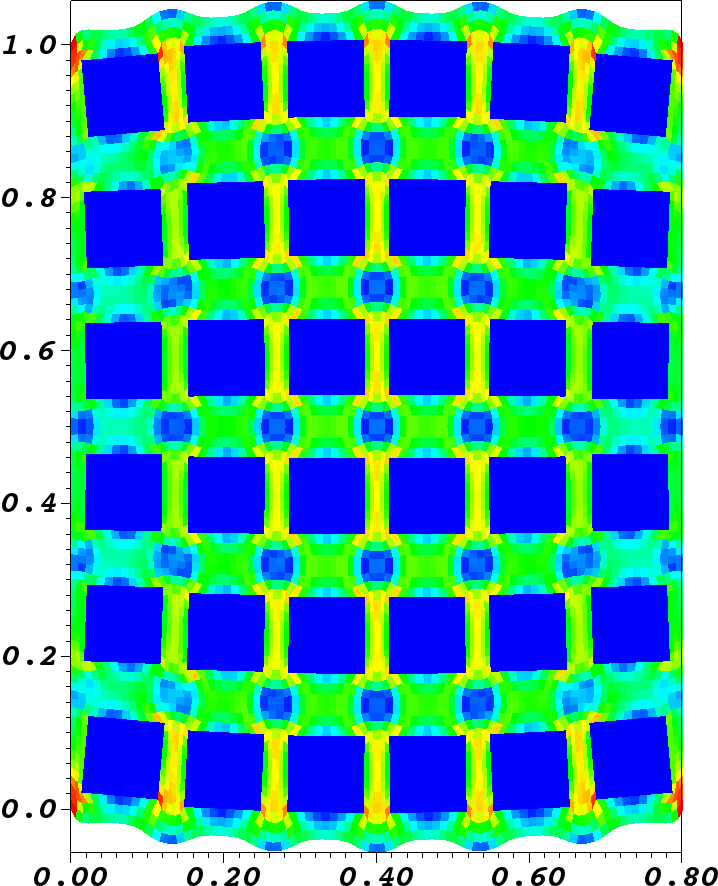
\includegraphics[width=\textwidth]{figures/MG/ElasticityCompressTrim}
            \caption{\scriptsize Initial solution.}\label{fig:elast-initial}
          \end{subfigure} ~
          \begin{subfigure}[b]{0.18\textwidth}
            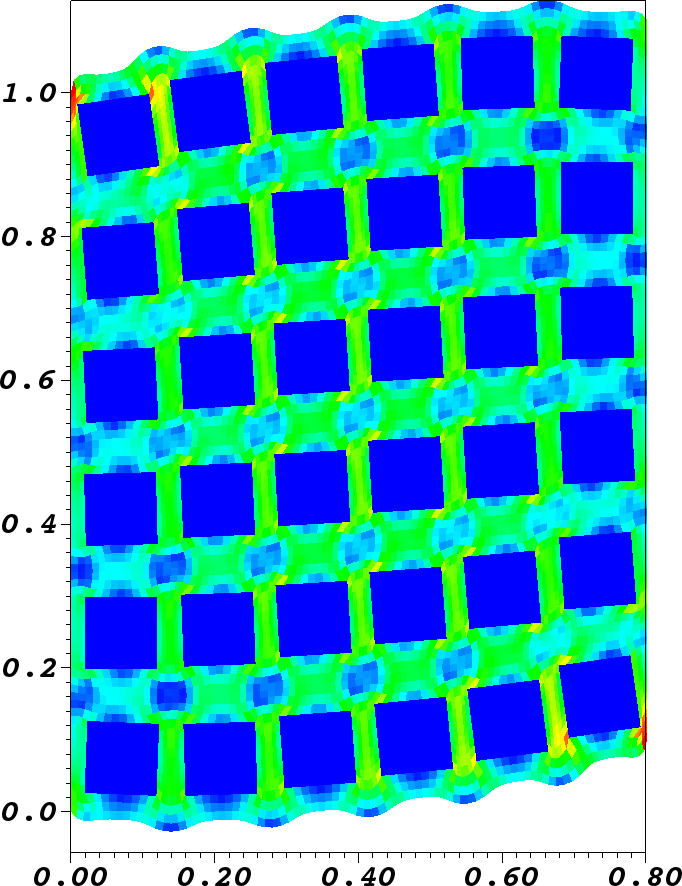
\includegraphics[width=\textwidth]{figures/MG/ElasticityCompressShearTrim}
            \caption{\scriptsize Increment.}\label{fig:elast-increment}
          \end{subfigure} ~
          \begin{subfigure}[b]{0.28\textwidth}
            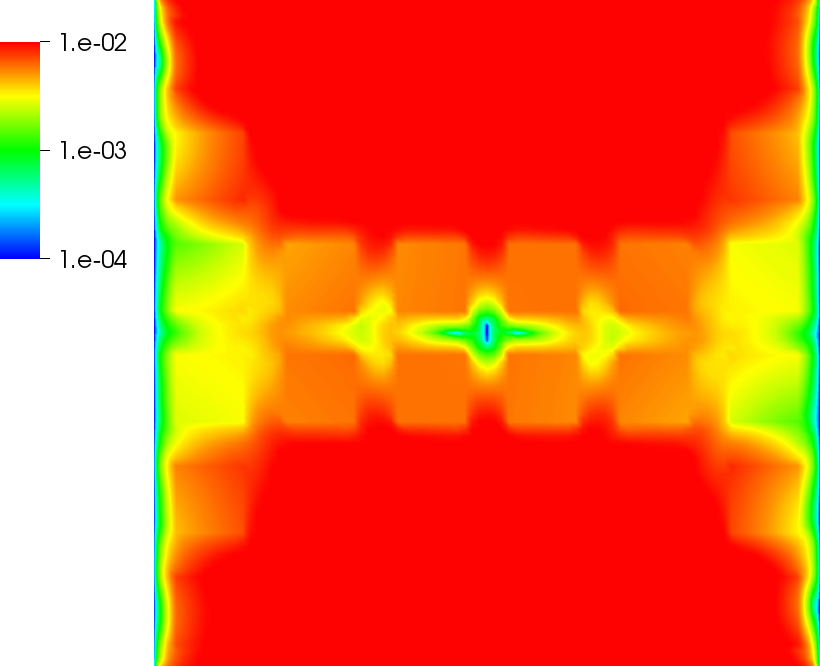
\includegraphics[width=\textwidth]{figures/MG/ElasticityCompressErrorNoTauTrim}
            \caption{\scriptsize Smoothed error, no $\tau$.}\label{fig:elast-error-notau}
          \end{subfigure} ~
          \begin{subfigure}[b]{0.28\textwidth}
            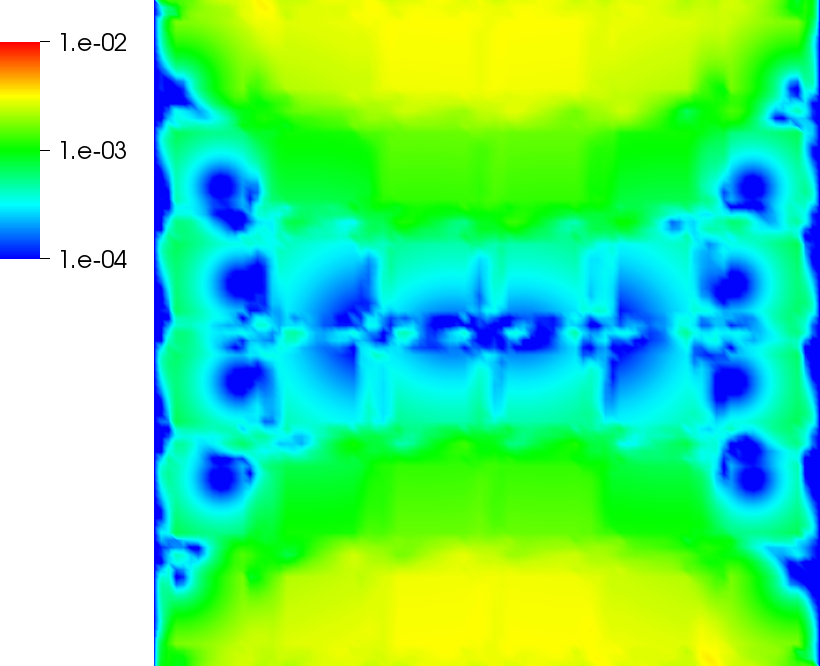
\includegraphics[width=\textwidth]{figures/MG/ElasticityCompressErrorTauTrim}
            \caption{\scriptsize Smoothed error, $\tau$.}\label{fig:elast-error-tau}
          \end{subfigure}
          \caption{Heterogeneous strain test using 2-level multigrid with coarsening factor of $3^2$.
            The coarse (respectively fine) grid has 3 (9) $Q_1$ elements across each block and 2 (6) elements across each gap.
            Panes (a) and (b) show the deformed body colored by strain.
            The initial problem of compression by 0.2 from the right is solved (a) and $\tau = A^H \hat I_h^H u^h - I_h^H A^h u^h$ is computed.
            Then a shear increment of 0.1 in the $y$ direction is added to the boundary condition, and the coarse-level problem is resolved, interpolated to the fine-grid, and a post-smoother is applied.
            When the coarse problem is solved without a $\tau$ correction (c), the displacement error is nearly $10\times$ larger than when $\tau$ is included in the right hand side of the coarse problem (d).
          }\label{fig:tau-valid}
        \end{figure}
      \end{block}
      \vspace{-2em}
      \begin{block}{Status}
        In PETSc: \texttt{src/ts/examples/tutorials/ex-seaice.c}, $Q_1$ discretization, FAS and geometric MG.
        Outstanding tasks:
        \begin{itemize}
        \item restrict active process set on coarse grids
        \item nonlinear Gauss-Seidel smoother
        \item unstructured geometric multigrid (almost complete)
        \item couple into thickness and concentration
        \item $\tau$ adaptivity to avoid most work in compressive regions
        \end{itemize}
      \end{block}
      \vspace{-2em}
      \begin{block}{References}
        \scriptsize
        % \nocite{brandt1994multigrid,bkmms2012}
        \begin{minipage}{\textwidth}
          \begin{multicols}{2}
            \bibliography{$HOME/jedbib/jedbib,$PETSC_DIR/src/docs/tex/petsc,$PETSC_DIR/src/docs/tex/petscapp,$HOME/proposals/navy-sea-ice/seaice}
          \end{multicols}
        \end{minipage}
      \end{block}
    \end{column}
  \end{columns}
\end{frame}
\end{document}

        % Recursive application of a technique called \emph{segmental refinement}, in which the fine grid state is populated on the fly from the coarser grid followed by smoothing, permits solution of problems using only poly-logarithmic memory, provided that the right hand side and coefficients are similarly compressible.
        % For highly heterogenous problems, the constants associated with this aggressive memory reduction become large, and we have to choose which ingredients are most crucial to a robust multigrid cycle.
        % \begin{description}
        % \item[Solution state] is small and frequently needed in complete form due to coupling to other equations and time-dependence.
        %   It is relatively expensive to reconstruct on the fly, especially on multiple coarse levels.
        % \item[Grid transfer operators] (coarse basis functions) are a critical ingredient for robust multigrid and also expensive to reconstruct in each visit.
        % \item[Coarse operators] provide a systematic compression of fine-scale heterogeneity.
        %   With a fast coarsening rate, coarse grid operators are relatively affordable.
        % \item[Fine grid operators] typically consume significantly more memory than the rest of the multigrid hierarchy, are performance-limited by memory bandwidth, and too expensive to reassemble for highly nonlinear problems.
        % \end{description}

%%%%%%%%%%%%%%%%%%%%%%%%%%%%%%%%%%%%%%%%%%%%%%%%%%%%%%%%%%%%%%%%%%%%%%%%%%%%%%%%%%%%%%%%%%%%%%%%%%%% 
%%% Local Variables: 
%%% mode: latex
%%% TeX-PDF-mode: t
%%% End: 


% Reference configuration:
%  mpirun.hydra -n 4 ./ex-seaice -snes_monitor -da_grid_x 21 -da_grid_y 21 -da_refine 4 -L 2e5,2e5 -snes_converged_reason -ts_monitor_solution_vtk 'si-%03d.vts' -snes_max_it 150 -ts_dt 1e-1 -ts_adapt_basic_clip 0.1,4 -ts_adapt_monitor -ts_atol 1e-3 -ts_rtol 1e-3 -ts_type arkimex -ts_arkimex_type 1bee -ksp_converged_reason -water_speed 0.01 -ts_adapt_dt_max 1e3 -pc_type mg

% mpirun.hydra -n 4 ./ex-seaice -snes_monitor -da_grid_x 21 -da_grid_y 21 -da_refine 4 -L 2e5,2e5 -snes_converged_reason -ts_monitor_solution_vtk 'si-%03d.vts' -snes_max_it 150 -ts_dt 1e-1 -ts_adapt_basic_clip 0.1,4 -ts_adapt_monitor -ts_atol 1e-3 -ts_rtol 1e-3 -ts_type arkimex -ts_arkimex_type 1bee -ksp_converged_reason -water_speed 0.01 -ts_adapt_dt_max 1e3 -snes_type fas -fas_levels_snes_type newtonls -fas_levels_snes_linesearch_type l2 -fas_levels_snes_max_it 5 -fas_levels_ksp_max_it 1 -fas_levels_ksp_type richardson -fas_levels_pc_type sor -fas_levels_ksp_convergence_test skip -fas_levels_snes_convergence_test skip -fas_levels_pc_sor_omega 1 -ts_max_steps 2

